\documentclass[10pt,twocolumn]{article}
\usepackage{geometry}
\geometry{verbose,headsep=3cm,tmargin=2.5cm,bmargin=2.5cm,lmargin=2.0cm,rmargin=2.0cm}
\usepackage{graphicx}
\usepackage{xcolor}
\usepackage[font=small]{caption}
\usepackage{amsmath,amssymb,latexsym}
\usepackage{marvosym}
\usepackage{url}
\usepackage{lipsum}
\usepackage{bm}
\usepackage{float}
\usepackage[english]{babel}
\usepackage{caption}
%\usepackage{subfigure}
\usepackage{subcaption}
\usepackage{subfloat}
\usepackage{hyperref}
\usepackage{epsf}
\usepackage{float}
\usepackage{mathpazo}
\usepackage{pifont}
\usepackage{graphicx}
%\usepackage{subfig}
\usepackage{wrapfig}
\usepackage{multicol}
\usepackage{enumitem}
\usepackage{xcolor}
\usepackage{framed}
\usepackage[utf8]{inputenc}
% Document font:
\usepackage{charter}
\graphicspath{{DWGs/}}
\newcommand*{\addheight}[2][.5ex]{%
  \raisebox{0pt}[\dimexpr\height+(#1)\relax]{#2}%
}

\begin{document}

\twocolumn[{
\begin{@twocolumnfalse}

  \begin{center}
%\textcolor{lgray}
    \vskip-5em

    \hfill
    \fontsize{10}{10}\selectfont {\textit{Bruxelles, January 2019}}

    \vskip2ex
    
	\vspace{5ex}
	
    \fontsize{24}{10}\selectfont {Underdetermined linear systems}
    
    \fontsize{18}{10}\selectfont {a short story with some code}



  \noindent%
    
\vskip1ex

{\rule{\textwidth}{0.5pt}}

  \end{center}
  
    \fontsize{7}{10}\selectfont {This work is licensed under the Creative Commons Attribution-NonCommercial-ShareAlike 4.0 International (CC BY-NC-SA 4.0) license.}

\vspace{6mm}

\end{@twocolumnfalse}
}]

\setlength{\parindent}{0cm}

\vspace{10mm}

\setlength{\parindent}{0cm}

\fontsize{14}{10}\selectfont {Kamila Zdybał}

\vspace{2mm}

\fontsize{8}{10}\selectfont {\textit{Université libre de Bruxelles, kamila.zdybal@ulb.ac.be}}

\fontsize{8}{10}\selectfont {\textit{camillejr.github.io/science-docs, kamila.zdybal@gmail.com}}

\vspace{2mm}



\section*{Preface}



\,\,

This document is still in preparation. Please feel free to contact me with any suggestions, corrections or comments.

\section*{Keywords}

\textit{underdetermined linear systems, linear algebra, matrix decomposition, matrix approximation}

\tableofcontents

\section{Introduction}

For an undertermined linear system (where matrix $\bm{A}$ is size $(n \times m)$ and $n<m$):

\begin{equation}
\bm{A} x = b
\end{equation}


an infinite number of solutions exists. MATLAB implements various methods of computing possible solutions for $x$. In this paper we investigate the differences in the available solutions by analyzing their histograms. Four methods were selected: backslash \texttt{\char`\\} operator, computing a pseudo-inverse \texttt{pinv()}, and two least-squares algorithms \texttt{lsqnonneg()} and \texttt{lsqr()}.

\section{Matlab example}

We focus on an example where matrix $\bm{A}$ is size $(100 \times 500)$ and a vector $b$ is size $(100 \times 1)$; both are populated by normally distributed random numbers.

\begin{figure}[H]
\centering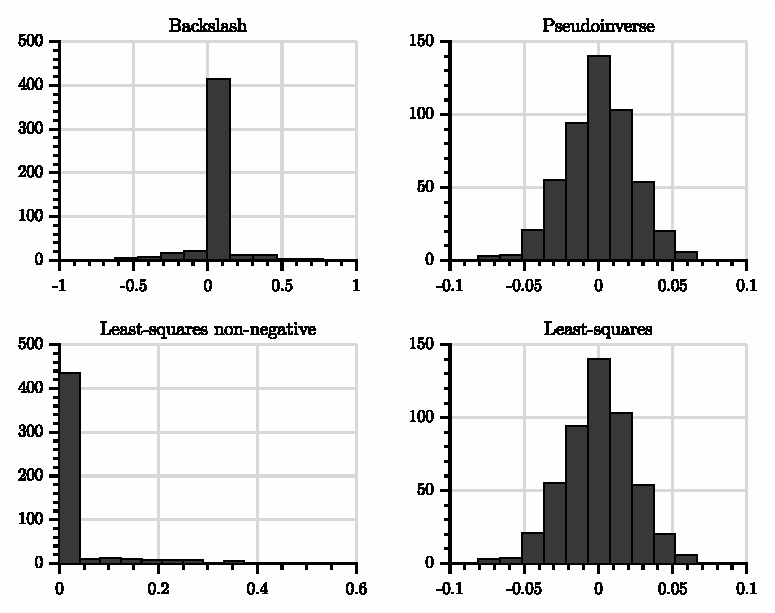
\includegraphics[width=8cm]{DWGs/histograms.eps}
\caption{Histograms of four solutions to an undetermined linear system.}			
\label{fig:histograms}
\end{figure}







\section{Possible applications}


\newpage


\thebibliography{}

\bibitem{Kutz} Nathan Kutz, \textit{Data Driven Discovery of Dynamical Systems and PDEs}, an online lecture 

\bibitem{Strang} Gilbert Strang, \textit{Introduction to Linear Algebra}, Fifth Edition, 2016

 \label{bib:pope}


\end{document}
